\chapter{Hậu xử lý kết quả}
Dữ liệu ảnh 3-chiều sau khi được dự đoán bởi mạng học sâu sẽ là một mảng 3-chiều số thực có giá trị trong đoạn $[0,1]$. Mảng này sẽ được chúng tôi tiếp tục xử lý để ra kết quả cuối cùng có giá trị nhất. Để giảm thiểu thời gian tính toán và đúng với tinh thần ứng dụng mạng học sâu cho phân đoạn ảnh, các bước hậu xử lý của chúng tôi chỉ sử dụng các thao tác đơn giản gồm: loại bỏ các khối nhiễu, lấp đầy các lỗ trống trong khối.
\section{Đánh nhãn vùng liên thông}
Đánh nhãn vùng liên thông (Connected-component labeling) là tác vụ cơ sở để chúng tôi thực hiện hai thao tác hậu xử lý là loại bỏ khối và lấp đầy khối. Tác vụ đánh nhãn này thường được sử dụng để xử lý các ảnh nhị phân cho các ứng dụng trong lĩnh vực thị giác máy tính. Tuy nhiên ảnh màu và ảnh có số chiều nhiều hơn hai vẫn có thể sử dụng giải pháp này.\\
Các giải thuật đánh nhãn vùng liên thông coi ảnh đầu vào là một đồ thị, điểm ảnh là đỉnh, mỗi điểm ảnh có cạnh với các điểm lân cận của điểm đó. Tuỳ vào bài toán mà người ta quy định các cạnh của một đỉnh. Mục tiêu của giải thuật là tìm ra các tập hợp các điểm ảnh nằm gần nhau và có giá trị bằng nhau. Sau đây chúng tôi sẽ trình bày hai giải thuật để đánh nhãn vùng liên thông là: một thành phần trong mỗi thời điểm (one component at a time) và hai vòng (two-pass).
\subsection{Giải thuật một thành phần trong mỗi thời điểm}
Đây là giải thuật cơ bản và dễ nghĩ tới nhất. Với giải thuật này, từng điểm ảnh sẽ được duyệt, sau đó kiểm tra tất cả các điểm liên thông và cùng giá trị với điểm ảnh này, lưu chúng lại ở dạng ma trận sao cho các thành liên thông có cùng giá trị. Đây là một phần giải thuật phân đoạn của Vincent và Soille\cite{87344}. Giải thuật với ma trận đầu vào nhị phân có hai giá trị $0, 1$ có mã giả \ref{OCAAT}.\\
\begin{algorithm}
  \caption{Giải thuật một thành phần trong mỗi thời điểm}\label{OCAAT}
  \begin{algorithmic}[1]
    \Procedure{OCAAT}{Array $A[m,n]$}
    \State Array $B[m, n]$ = $0$ \Comment{Khởi tạo ma trận trả về, 0: chưa duyệt}
    \State Queue $q$ \Comment{Khởi tạo queue q rỗng}
    \State Integer $current\_label$ = $1$
    
    \For{$i = 0$ to $m$ }
        \For{$j = 0$ to $n$}
            \If{$A[i,j]$ == $1$ and $B[i,j]$ == $0$} \Comment{điểm (i,j) không phải nền và chưa duyệt}
                \State $B[i,j]$ = $current\_label$ \Comment{đánh nhãn điểm(i,j)}
                \State $q.push([i,j])$
            \Else
                \State continue
            \EndIf
            \While {$q$ is not empty}
                \State $pixel$ = $q.pop()$
                \State $neighbors$ = $get\_neighbors(pixel)$
                \For {each $neighbor$ in $neighbors$}
                    \If{$A[neighbor]$ == $1$ and $B[neighbor]$ == $0$}
                        \State $B[i,j]$ = $current\_label$
                        \State $q.push(neighbor)$
                    \EndIf
                \EndFor
            \EndWhile
            \State $current\_label$ += $1$
        \EndFor   
    \EndFor
    \Return $B, current\_label$
    \EndProcedure
  \end{algorithmic}
\end{algorithm}
Giải thuật \ref{OCAAT} có thể mở rộng trên nhiều chiều và nhiều giá trị điểm ảnh khác nhau. Trong bài toán xác định vùng gan, chúng tôi sử dụng giải thuật đánh nhãn trong không gian 3-chiều và hai giá trị đã được làm tròn thành $0,1$.

\subsection{Giải thuật hai vòng}
Một giải thuật khác để đánh nhãn cho các vùng được trình bày trong \ref{twopass}. Tuỳ giải thuật \ref{twopass} mà hàm $find$ và $union$ sẽ được sử dụng với một cấu trúc dữ liệu đặc biệt để việc chia và gộp các vùng nhanh hơn.
\begin{algorithm}
  \caption{Giải thuật hai vòng}\label{twopass}
  \begin{algorithmic}[1]
    \Procedure{TwoPass}{Array $A[m,n]$}
    \State Array $B[m, n] = 0$ \Comment{Khởi tạo ma trận trả về, 0: chưa duyệt}
    \State Dict $dict = \{\}$
    \State Integer $next\_label = 1$
    
    \For{$i = 0$ to $m$ }
        \For{$j = 0$ to $n$}
            \If{$A[i,j] != 0$}
                \State $neighbors$ = $get\_neighbors\_foreground(A[i,j])$
                \If{$neighbors$ is empty}
                    \State $dict[next\_label]$ = $set()$
                    \State $B[i,j]$ = $next\_label$
                    \State $next\_label$ += $1$
                \Else
                    \State $L$ = $getLabels(neigbors)$
                    \State $B[i,j]$ = $min(L)$
                    \For {each $label$ in $L$}
                        \State $dict[label]$ += $union(dict[label], L)$
                    \EndFor
                \EndIf
            \EndIf
        \EndFor   
    \EndFor
    \For{$i = 0$ to $m$ }
        \For{$j = 0$ to $n$}
            \If{$A[i,j]$ != $0$}
                \State $B[i,j]$ = $find(labels[i,j])$
            \EndIf
        \EndFor   
    \EndFor
    \State \Return $B, next\_label$
    \EndProcedure
  \end{algorithmic}
\end{algorithm}
\section{Loại bỏ khối}
Với bài toán phân đoạn lá gan, để kết quả có thể sử dụng các thao tác hậu xử lý thì kết quả đó phải đạt tới một mức độ chính xác nhất định. Khi đó trên dữ liệu 3-chiều sẽ có một thành phần liên thông lớn nhất chính là lá gan, còn những thành phần liên thông khác thông thường sẽ không trùng với lá gan vì vậy sẽ bị loại bỏ. Qua thực nghiệm, thao tác loại bỏ các thành phần liên thông khác lớn nhất bằng Giải thuật \ref{remove_components} cho kết quả có độ chính xác cao hơn.\\
\begin{algorithm}
  \caption{Giải thuật của chúng tôi loại bỏ các thành phần nhiễu}\label{remove_components}
  \begin{algorithmic}[1]
    \Procedure{remove\_components}{Array $A[m,n]$}
    \State Array $B[m,n]$ = $0$
    \State Integer $numComponents$ = $0$
    \State $B, numComponents$ = $labels(A)$ \Comment{Sử dụng hàm đánh nhãn ở mục trước}
    \State List<Integer> $counts$
    \For{$i = 0$ to $numComponents$ -$1$}
        \State $counts[i]$ = $count\_pixel\_equal(B, i)$
    \EndFor
    \State Integer $choose$ = $index\_max(counts)$
    \For{each $P$ in $B$}
        \If{$P$ != $choose$}
            \State $P$ = $0$ \Comment{Gán điểm P là nền}
        \Else
            \State $P$ = $1$
        \EndIf
    \EndFor
    
    \State \Return $B$
    \EndProcedure
  \end{algorithmic}
\end{algorithm}

\begin{figure*}
  \centering
    \subfigure[Một lát cắt dự đoán trước khi hậu xử lý.]{%
    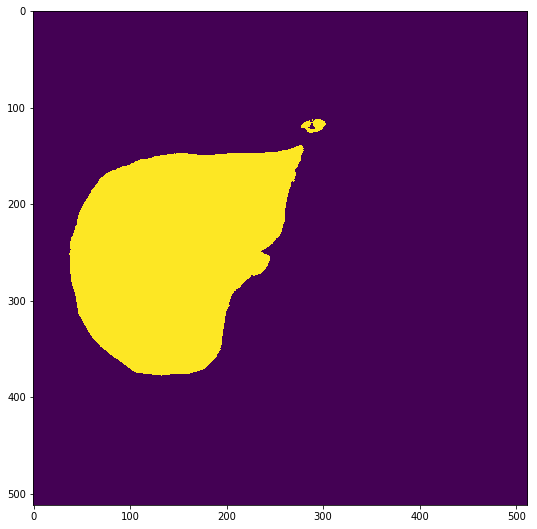
\includegraphics[width=0.45\textwidth]{Images/no_fill_result.png}%
    \label{fig:no_post_pro}%
    }
    \subfigure[Một lát cắt dự đoán sau khi hậu xử lý.]{%
    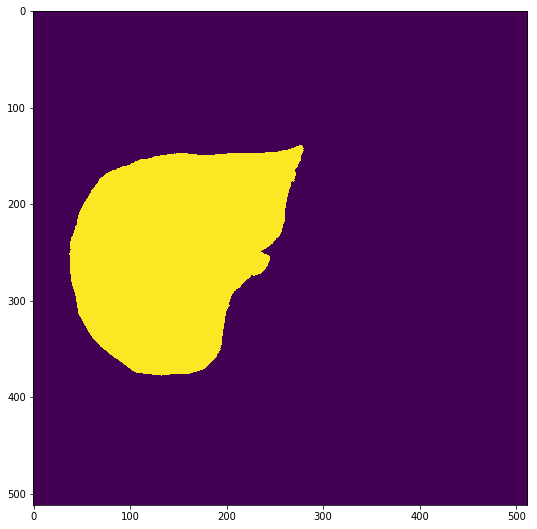
\includegraphics[width=0.45\textwidth]{Images/filled_result.png}%
    \label{fig:post_pro}%
    }% 
  \caption{Thay đổi của một dự đoán trước và sau hậu xử lý}
  \label{fig:post_process}
\end{figure*}

\section{Lấp đầy khối}
Sau khi có được kết quả dự đoán, bên cạnh loại bỏ các khối dự đoán nhiễu, chúng tôi thực hiện thao tác lấp đầy khối dự đoán chính là lá gan. Qua thực nghiệm, kết quả dự đoán sau khi được xử lý bằng cách này cho độ chính xác cao hơn và hình ảnh hiển thị rõ ràng hơn. Hiện tại đã có nhiều thư viện của python hỗ trợ thao tác này ví dụ như \textbf{scipy} với hàm \textbf{ndimage.binary\_fill\_holes}. Tuy nhiên, chúng tôi vẫn tìm tòi được một giải thuật xử lý thao tác này bằng cách sửa đổi Giải thuật \ref{OCAAT}.

\begin{algorithm}
  \caption{Giải thuật của chúng tôi để lấp đầy khối}\label{OCAAT2}
  \begin{algorithmic}[1]
    \Procedure{fill\_hole}{Array $A[m,n]$}
    
    \State Array $B[m, n]$ = $1$ \Comment{Khởi tạo ma trận trả về, 1: chưa duyệt}
    \State Queue $q$ \Comment{Khởi tạo queue q rỗng}
    
    \For{$(i,j)$ is the address of pixels on the border} \Comment{Lấy những điểm trên biên}
        \If{$A[i,j]$ == $0$ and $B[i,j]$ == $1$} \Comment{điểm (i,j) là nền và chưa duyệt}
            \State $B[i,j]$ = $0$ \Comment{ghi nhận điểm nền}
            \State $q.push([i,j])$
        \Else
            \State continue
        \EndIf
        \While {$q$ is not empty}
            \State $pixel$ = $q.pop()$
            \State $neighbors$ = $get\_neighbors(pixel)$
            \For {each $neighbor$ in $neighbors$}
                \If{$A[neighbor]$ == $0$ and $B[neighbor]$ == $1$}
                    \State $B[i,j]$ = $0$
                    \State $q.push(neighbor)$
                \EndIf
            \EndFor
        \EndWhile
    \EndFor
    \State \Return $B, current\_label$
    \EndProcedure
  \end{algorithmic}
\end{algorithm}